% ==================================================================================
% W-DsgDetr++ Method — Detailed Technical Report
% Target Venue: NeurIPS
% ==================================================================================
\documentclass{article}

% Uncomment if neurips_2026.sty is available
% \usepackage[preprint]{neurips_2026}
% Fallback to standard margins if neurips is unavailable:
\usepackage[margin=1in]{geometry}

\usepackage[utf8]{inputenc}
\usepackage{amsmath,amssymb,amsfonts}
\usepackage{graphicx}
\usepackage{booktabs}
\usepackage{algorithm}
\usepackage{algpseudocode}
\usepackage{bm}
\usepackage{xcolor}
\usepackage{tikz}
\usetikzlibrary{arrows.meta,positioning,shapes.geometric,fit,calc,backgrounds}

\newcommand{\mR}{\mathbb{R}}
\newcommand{\op}[1]{\operatorname{#1}}
\newcommand{\mat}[1]{\bm{#1}}

\title{W-DsgDetr++: Fully Enhanced World Scene Graph Generation with Tracking}
\author{Anonymous Authors}

\begin{document}

\maketitle

% ====================================================================================
\section{Introduction}
\label{sec:intro}
% ====================================================================================

The W-DsgDetr++ architecture represents the most feature-rich baseline adaptation in our study. It builds upon the W-DsgDetr model by activating every available shared encoder module. In addition to the explicit per-object tracking provided by the TemporalObjectEncoder, W-DsgDetr++ incorporates camera-relative spatial representations (ObjectSpatialEncoder), 3D object dynamics (ObjectMotionEncoder), and a novel ego-motion sequence model (CameraTemporalEncoder). 

This comprehensive suite of features tests the upper limits of performance achievable within a passive-memory (LKS Buffer) paradigm prior to introducing the masked auto-encoder retrieval mechanisms of the WorldWise model. W-DsgDetr++ utilizes a FasterRCNN-ResNet50 backbone.

% ====================================================================================
\section{Pipeline Overview}
\label{sec:pipeline}
% ====================================================================================

Figure~\ref{fig:pipeline_wdsgdetr_pp} illustrates the complete dataflow. Features are aggressively enriched with multiple structural, spatial, and dynamic encodings before undergoing explicit temporal object tracking, global spatial reasoning, and temporal edge attention.

\begin{figure}[h]
\centering
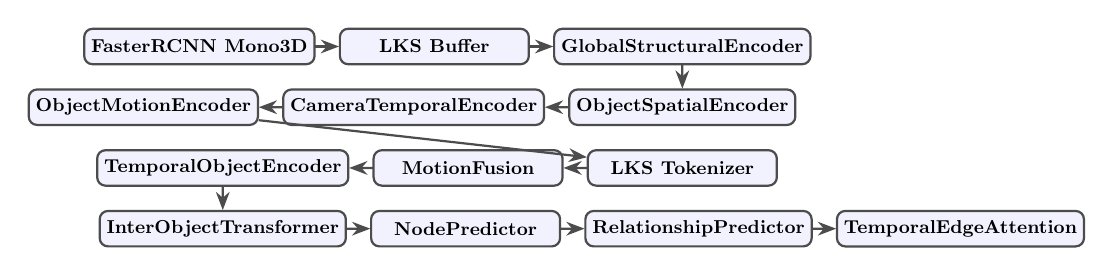
\begin{tikzpicture}[
  scale=0.75, transform shape, >=Stealth,
  block/.style={draw=black!70, rounded corners=3pt, line width=0.8pt, fill=blue!5, minimum width=3.2cm, minimum height=0.6cm, font=\small\bfseries, align=center},
  arrow/.style={->, thick, black!70}
]

\node[block] (mono) {FasterRCNN Mono3D};
\node[block, right=0.4cm of mono] (buffer) {LKS Buffer};
\node[block, right=0.4cm of buffer] (gse) {GlobalStructuralEncoder};
\node[block, below=0.4cm of gse] (ose) {ObjectSpatialEncoder};
\node[block, left=0.4cm of ose] (cte) {CameraTemporalEncoder};
\node[block, left=0.4cm of cte] (ome) {ObjectMotionEncoder};
\node[block, below=0.4cm of ose] (tok) {LKS Tokenizer};
\node[block, left=0.4cm of tok] (fuse) {MotionFusion};
\node[block, left=0.4cm of fuse] (toe) {TemporalObjectEncoder};
\node[block, below=0.4cm of toe] (iot) {InterObjectTransformer};
\node[block, right=0.4cm of iot] (np) {NodePredictor};
\node[block, right=0.4cm of np] (rp) {RelationshipPredictor};
\node[block, right=0.4cm of rp] (tea) {TemporalEdgeAttention};

\draw[arrow] (mono) -- (buffer);
\draw[arrow] (buffer) -- (gse);
\draw[arrow] (gse) -- (ose);
\draw[arrow] (ose) -- (cte);
\draw[arrow] (cte) -- (ome);
\draw[arrow] (ome) -- (tok);
\draw[arrow] (tok) -- (fuse);
\draw[arrow] (fuse) -- (toe);
\draw[arrow] (toe) -- (iot);
\draw[arrow] (iot) -- (np);
\draw[arrow] (np) -- (rp);
\draw[arrow] (rp) -- (tea);

\end{tikzpicture}
\caption{The W-DsgDetr++ pipeline. It incorporates all available spatial and temporal encoders, including explicit ego-motion tracking (CameraTemporalEncoder).}
\label{fig:pipeline_wdsgdetr_pp}
\end{figure}


% ====================================================================================
\section{LKS Memory Buffer and Structural Encoding}
\label{sec:lks_gse}
% ====================================================================================

W-DsgDetr++ maintains persistent visual states using the LKS Buffer $\mat{m}_n^{(t)}$ and calculates staleness $\Delta_n^{(t)}$. 

The \emph{GlobalStructuralEncoder} generates 3D geometric tokens. The 8 OBB corners are centered ($\bar{\mat{c}}_n$), flattened, concatenated, and projected via MLP:
\begin{equation}
    \mat{g}_n = \op{MLP}_{\text{obj}}\bigl([\op{flatten}(\mat{c}_{n,i} - \bar{\mat{c}}_n) \;\|\; \bar{\mat{c}}_n]\bigr) \in \mR^{d_{\text{struct}}}.
    \label{eq:gse_obj}
\end{equation}

% ====================================================================================
\section{Camera and Motion Encoders}
\label{sec:camera_motion}
% ====================================================================================

\subsection{ObjectSpatialEncoder}
Camera-relative positions are computed from the extrinsic matrix $\mat{T} = [\mat{R}\,|\,\boldsymbol{\tau}]$. A global camera token $\mat{c}_{\text{cam}}$ is formed from $\op{MLP}([\op{6D}(\mat{R}) \;\|\; \boldsymbol{\tau}])$. For each object, the direction $\mat{d}_n = \bar{\mat{c}}_n - \boldsymbol{\tau}$, view alignment $\alpha_n$, and azimuth $\beta_n$ are projected:
\begin{equation}
    \mat{c}_n = \op{MLP}\bigl([\log\|\mat{d}_n\|,\;\alpha_n,\;\beta_n^{\sin},\;\beta_n^{\cos}]\bigr) \in \mR^{d_{\text{camera}}}.
    \label{eq:cam_per_obj}
\end{equation}

\subsection{CameraTemporalEncoder}
To capture ego-motion (e.g., panning, orbiting), we compute relative camera poses between consecutive frames:
\begin{align}
    \mat{R}_{\text{rel}}^{(t)} &= \mat{R}_t \mat{R}_{t-1}^{\!\top}, \label{eq:rel_rot} \\
    \boldsymbol{\tau}_{\text{rel}}^{(t)} &= \boldsymbol{\tau}_t - \mat{R}_{\text{rel}}^{(t)}\boldsymbol{\tau}_{t-1}. \label{eq:rel_trans}
\end{align}
The sequence of relative poses is encoded via self-attention:
\begin{equation}
    \mat{e}_t = \op{EgoAttn}\bigl(\{\op{MLP}([\op{6D}(\mat{R}_{\text{rel}}^{(\tau)}) \;\|\; \boldsymbol{\tau}_{\text{rel}}^{(\tau)}]) + \mat{e}_{\tau}\}_{\tau=0}^{T-1}\bigr),
    \label{eq:ego_motion}
\end{equation}
yielding an ego-motion token $\mat{e}_t \in \mR^{d_{\text{camera}}}$ for each frame.

\subsection{ObjectMotionEncoder}
Per-object 3D velocity $\mat{v}_n^{(t)}$ and acceleration $\mat{a}_n^{(t)}$ are computed via finite differences of OBB centers. Combined with camera-relative velocity $\mat{R}^{\!\top}\mat{v}_n$, the 11-dim feature is projected to $\mat{\mu}_n^{(t)} \in \mR^{d_{\text{motion}}}$.


% ====================================================================================
\section{Tokenizer and Fusion}
\label{sec:fusion}
% ====================================================================================

The Tokenizer aggregates geometry, buffered features, spatial encodings, and staleness:
\begin{equation}
    \mat{x}_n^{(t)} = \op{FusionProj}\bigl([\mat{g}_n^{(t)} \;\|\; \mat{m}_n^{(t)} \;\|\; \mat{c}_n^{(t)} \;\|\; \log(\Delta_n^{(t)} + 1)]\bigr) \in \mR^{d_{\text{model}}}.
    \label{eq:tokenizer}
\end{equation}
Motion and ego-motion are then fused. The ego-motion token $\mat{e}_t$ is broadcast to all $N$ objects in frame $t$:
\begin{equation}
    \hat{\mat{x}}_n^{(t)} = \op{LayerNorm}\bigl(\op{Linear}([\mat{x}_n^{(t)} \;\|\; \mat{\mu}_n^{(t)} \;\|\; \mat{e}_t])\bigr).
    \label{eq:fusion}
\end{equation}


% ====================================================================================
\section{Temporal Tracking and Spatial Reasoning}
\label{sec:tracking}
% ====================================================================================

\subsection{TemporalObjectEncoder}
Each object's temporal sequence is processed by a Transformer encoder to interpolate features across time:
\begin{equation}
    \tilde{\mat{X}}_n = \op{TransformerEncoder}\bigl(\{\hat{\mat{x}}_n^{(t)} + \mat{PE}_{\text{sin}}(t)\}_{t=1}^T,\; \text{mask}=\text{pad\_mask}_n\bigr).
    \label{eq:toe}
\end{equation}

\subsection{InterObjectTransformer}
The refined representations undergo global spatial reasoning using additive pairwise spatial positional encodings $\mat{S}^{(t)}$:
\begin{equation}
    \mat{H}^{(t)} = \op{TransformerEncoder}\bigl(\tilde{\mat{X}}^{(t)} + \mat{S}^{(t)},\; \text{mask}=\overline{\mat{v}}^{(t)}\bigr).
    \label{eq:iot}
\end{equation}


% ====================================================================================
\section{Predictors and Temporal Edge Attention}
\label{sec:predictors}
% ====================================================================================

Node classes are predicted via an MLP ($\hat{\mat{Y}}^{\text{obj}}$). Edge tokens $\mat{r}_{po}$ are formed from subject/object features, union features, and class semantic embeddings, then processed by intra-frame self-attention.

Finally, \emph{TemporalEdgeAttention} applies cross-frame self-attention over each unique object pair's relationship tokens, using learned temporal positional embeddings $\mat{e}_\tau$:
\begin{equation}
    \tilde{\mat{r}}_{po}^{(t)} = \op{TemporalEncoder}\bigl(\{{\mat{r}}_{po}^{(\tau)} + \mat{e}_{\tau}\}_{\tau \in \mathcal{T}_{po}}\bigr).
    \label{eq:tea}
\end{equation}
Three MLP heads map $\tilde{\mat{r}}_{po}^{(t)}$ to attention, spatial, and contacting logits.


% ====================================================================================
\section{Loss Function}
\label{sec:loss}
% ====================================================================================

The total loss sums visible pair losses (clean GT) and unseen pair losses (VLM pseudo-labels with label smoothing and $\lambda_{\text{vlm}}$ weighting):
\begin{equation}
    \mathcal{L}_{\text{W-DsgDetr++}} = \sum_{r \in \{\text{att, spa, con}\}} \bigl(\mathcal{L}_{r}^{\text{vis}} + \mathcal{L}_{r}^{\text{unseen}}\bigr) + \mathcal{L}_{\text{node}}.
    \label{eq:loss}
\end{equation}


% ====================================================================================
\section{Algorithm: Forward Pass}
\label{sec:algorithm}
% ====================================================================================

\begin{algorithm}[h]
\caption{W-DsgDetr++ Forward Pass}
\begin{algorithmic}[1]
\Require $\mat{f}_{\text{all}}$ (visual), $\mat{C}_{\text{all}}$ (OBBs), $\mat{T}_{\text{all}}$ (camera)
\Ensure $\hat{\mat{y}}_{\text{att}}, \hat{\mat{y}}_{\text{spa}}, \hat{\mat{y}}_{\text{con}}$
\State $(\mat{m}_{\text{all}}, \bm{\Delta}_{\text{all}}) \gets \text{LKS\_Buffer}(\mat{f}_{\text{all}})$
\State $\mat{G}_{\text{all}} \gets \text{GlobalStructuralEncoder}(\mat{C}_{\text{all}})$
\State $\mat{c}_{\text{all}} \gets \text{ObjectSpatialEncoder}(\mat{T}_{\text{all}}, \mat{C}_{\text{all}})$
\State $\mat{e}_{\text{all}} \gets \text{CameraTemporalEncoder}(\mat{T}_{\text{all}})$
\State $\mat{\mu}_{\text{all}} \gets \text{ObjectMotionEncoder}(\mat{C}_{\text{all}}, \mat{T}_{\text{all}})$
\State $\mat{X} \gets \text{Tokenizer}(\mat{G}_{\text{all}}, \mat{m}_{\text{all}}, \mat{c}_{\text{all}}, \log \bm{\Delta}_{\text{all}})$
\State $\hat{\mat{X}} \gets \text{MotionFusion}(\mat{X}, \mat{\mu}_{\text{all}}, \mat{e}_{\text{all}})$
\State $\tilde{\mat{X}} \gets \text{TemporalObjectEncoder}(\hat{\mat{X}})$
\State $\mat{H} \gets \text{InterObjectTransformer}(\tilde{\mat{X}})$
\State $\hat{\mat{Y}}^{\text{obj}} \gets \text{NodePredictor}(\mat{H})$
\State $\mat{R} \gets \text{RelationshipFormationAndSelfAttention}(\mat{H}, \hat{\mat{Y}}^{\text{obj}})$
\State $\tilde{\mat{R}} \gets \text{TemporalEdgeAttention}(\mat{R})$
\State $(\hat{\mat{y}}_{\text{att}}, \hat{\mat{y}}_{\text{spa}}, \hat{\mat{y}}_{\text{con}}) \gets \text{PredictionHeads}(\tilde{\mat{R}})$
\State \Return $\hat{\mat{y}}_{\text{att}}, \hat{\mat{y}}_{\text{spa}}, \hat{\mat{y}}_{\text{con}}$
\end{algorithmic}
\end{algorithm}

\end{document}
